\documentclass{beamer}
\usepackage[backend=bibtex,style=numeric,sorting=none]{biblatex}
\usepackage{progressbar}
\usepackage[final]{listings}
\usepackage{graphicx}
\graphicspath{ {./images/} }

\addbibresource{main.bib}
\usetheme{AnnArbor}

\title{Container Security}
\subtitle{Bachelor's degree graduation project}
\author{Chih-Hsuan Yang}
\institute{National Sun Yat-sen University}
\date{\today}

\AtBeginSection[]{
    \begin{frame}
        \vfill
        \centering
        \begin{beamercolorbox}[sep=8pt,center,shadow=true,rounded=true]{title}
          \usebeamerfont{title}\insertsectionhead\par
        \end{beamercolorbox}
        \vfill
        \end{frame}
}

\definecolor{mygreen}{rgb}{0,0.6,0}
\definecolor{mygray}{rgb}{0.5,0.5,0.5}
\definecolor{mymauve}{rgb}{0.58,0,0.82}

% Code conf.
\lstset{ 
  backgroundcolor=\color{white},   % choose the background color; you must add \usepackage{color} or \usepackage{xcolor}; should come as last argument
  basicstyle=\ttfamily\footnotesize,% the size of the fonts that are used for the code
  breakatwhitespace=false,         % sets if automatic breaks should only happen at whitespace
  breaklines=true,                 % sets automatic line breaking
  captionpos=b,                    % sets the caption-position to bottom
  commentstyle=\color{mygreen},    % comment style
  deletekeywords={...},            % if you want to delete keywords from the given language
  escapeinside={\%*}{*)},          % if you want to add LaTeX within your code
  extendedchars=true,              % lets you use non-ASCII characters; for 8-bits encodings only, does not work with UTF-8
  frame=single,	                   % adds a frame around the code
  keepspaces=true,                 % keeps spaces in text, useful for keeping indentation of code (possibly needs columns=flexible)
  keywordstyle=\color{red},       % keyword style
  morekeywords={*,...},            % if you want to add more keywords to the set
  numbers=left,                    % where to put the line-numbers; possible values are (none, left, right)
  numbersep=5pt,                   % how far the line-numbers are from the code
  numberstyle=\tiny\color{mygray}, % the style that is used for the line-numbers
  rulecolor=\color{black},         % if not set, the frame-color may be changed on line-breaks within not-black text (e.g. comments (green here))
  showspaces=false,                % show spaces everywhere adding particular underscores; it overrides 'showstringspaces'
  showstringspaces=false,          % underline spaces within strings only
  showtabs=false,                  % show tabs within strings adding particular underscores
  stepnumber=1,                    % the step between two line-numbers. If it's 1, each line will be numbered
  stringstyle=\color{mymauve},     % string literal style
  tabsize=4,	                     % sets default tabsize to ˋ spaces
}


\begin{document}

\begin{frame}
    \titlepage
\end{frame}

\begin{frame}
    \frametitle{Outline}
    \tableofcontents
\end{frame}

% ======================Why this issue============================
\section{Why this issue}
\subsection{Story}
\begin{frame}
    \frametitle{AIS3 - mentor final exhibition}

    \begin{itemize}
        \item Kun-Yu Chen
              \begin{itemize}
                  \item The origin issue is too hard.
              \end{itemize}
        \item Tim Hsu
              \begin{itemize}
                  \item My "AIS3 mentor" in this year.
                  \item Working and interesting vector dot product.
              \end{itemize}
        \item Linux Kernel
              \begin{itemize}
                  \item 2020 Early, with jserv.
              \end{itemize}
        \item Program efficiency
              \begin{itemize}
                  \item Not only the big-O but also care about the impl.
              \end{itemize}
        \item Heavy dependence with container
              \begin{itemize}
                  \item Club, my works...
              \end{itemize}
    \end{itemize}

\end{frame}

\subsection{Modern critical issue}
\begin{frame}
    \frametitle{Microservices}
    \begin{itemize}
        \item Services are small in size, messaging-enabled, bounded by contexts, \
              autonomously developed, independently deployable, decentralized and \
              built and released with automated processes.\cite{Microservice_book}
        \item Scenario
        \item Share resources, load balance, sandbox and so on\dots
    \end{itemize}
\end{frame}

\begin{frame}
    \frametitle{DEFCON}
    \begin{itemize}
        \item DEFCON 26: Workshop\cite{DEFCON26_workshop}
        \item DEFCON 27: Workshop\cite{DEFCON27_workshop}
        \item BlackHat(USA) 2018: Conference\cite{BlackHat2018}
        \item BlackHat(USA) 2019: Conference\cite{BlackHat2019}
        \item BlackHat(USA) 2020: Conference\cite{BlackHat2020}
    \end{itemize}
\end{frame}


% ======================How this issue============================

\section{How this issue}
\subsection{Study}
\begin{frame}
    \frametitle{CVEs}
    \begin{itemize}
        \item Linux kernel
              \begin{itemize}
                  \item CVE-2016-5195 a.k.a. Dirty-CoW
                  \item CVE-2016-8655
                  \item CVE-2017-7308
                  \item CVE-2020-14386
              \end{itemize}
        \item Language feature
              \begin{itemize}
                  \item C, C++, Golang, Rust\dots
                  \item e.g.: gVisor
              \end{itemize}
        \item Container implementation
              \begin{itemize}
                  \item TBD
              \end{itemize}
    \end{itemize}
\end{frame}

% ======================Paper review============================

\section{Paper review}
\subsection{Papers}
\begin{frame}
    \frametitle{Have been read papers}
    \begin{itemize}
        \item Study of the Dirty Copy on Write, a Linux Kernel Memory Allocation Vulnerability\cite{Study_Dirty_Cow}
        \item Container Security: Issues, Challenges, and the Road Ahead\cite{Road_Ahead}
        \item Container Image Access Control Architecture to Protect Applications\cite{Access_Control_Architecture}
    \end{itemize}
\end{frame}

\begin{frame}
    \frametitle{To be read papers}
    \begin{itemize}
        \item Linux Kernel OS Local Root Exploit\cite{root_exploit}
        \item PINE: Optimizing Performance Isolation in Container Environments\cite{Optimizing}
        \item Study of Security Flaws in the Linux Kernel by Fuzzing\cite{Fuzzing}
    \end{itemize}
\end{frame}

\subsection{Dirty CoW}
\begin{frame}
    \frametitle{Dirty CoW overview}
    \lstinputlisting[language=C, linerange={106-107}, firstnumber=106]{../../apply/dirtyc0w.c}
\end{frame}

\begin{frame}
    \frametitle{Dirty CoW overview}
    \lstinputlisting[language=C, linerange={50-53,61-63,67-71}, firstnumber=50]{../../apply/dirtyc0w.c}
\end{frame}

\begin{frame}
    \frametitle{Dirty CoW overview}
    \lstinputlisting[language=C, linerange={33-39,45-48}, firstnumber=33]{../../apply/dirtyc0w.c}
\end{frame}

\subsection{Road ahead}
\begin{frame}
    \frametitle{Issues, Challenges and road ahead}
    \begin{itemize}
        \item There are no comprehensive surveys on container security.
        \item 4 types of protection
              \begin{itemize}
                  \item protecting a container from applications inside it
                  \item inter-container protection
                  \item protecting the host from containers
                  \item protecting containers from host
              \end{itemize}
        \item Available solutions:
              \begin{itemize}
                  \item Linux namespaces, CGroups, capabilities, seccomp, and LSMs
                  \item hardware solutions
              \end{itemize}
    \end{itemize}
\end{frame}

\subsection{Access control architecture}
\begin{frame}
    \frametitle{Access control architecture to protect applications}
    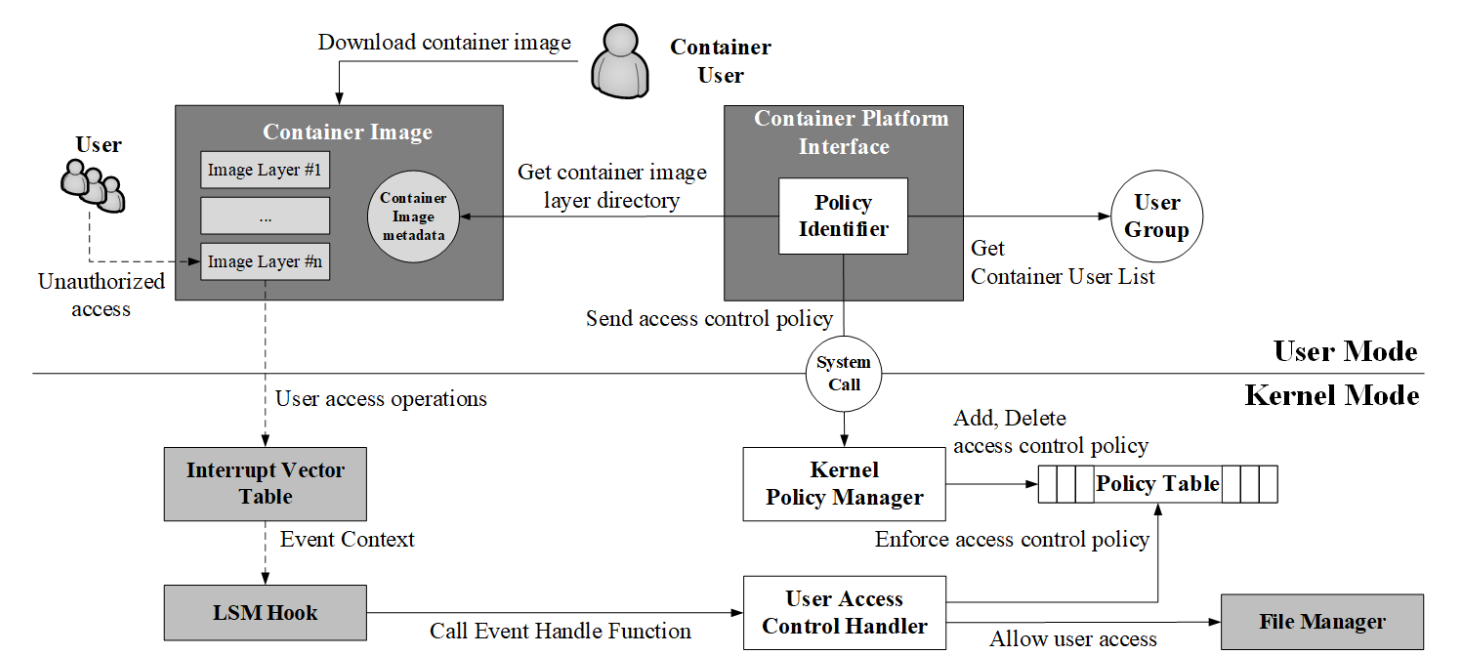
\includegraphics[width=\textwidth]{architecture.png}\cite{Access_Control_Architecture}
\end{frame}

\begin{frame}
    \frametitle{Access control architecture to protect applications}
    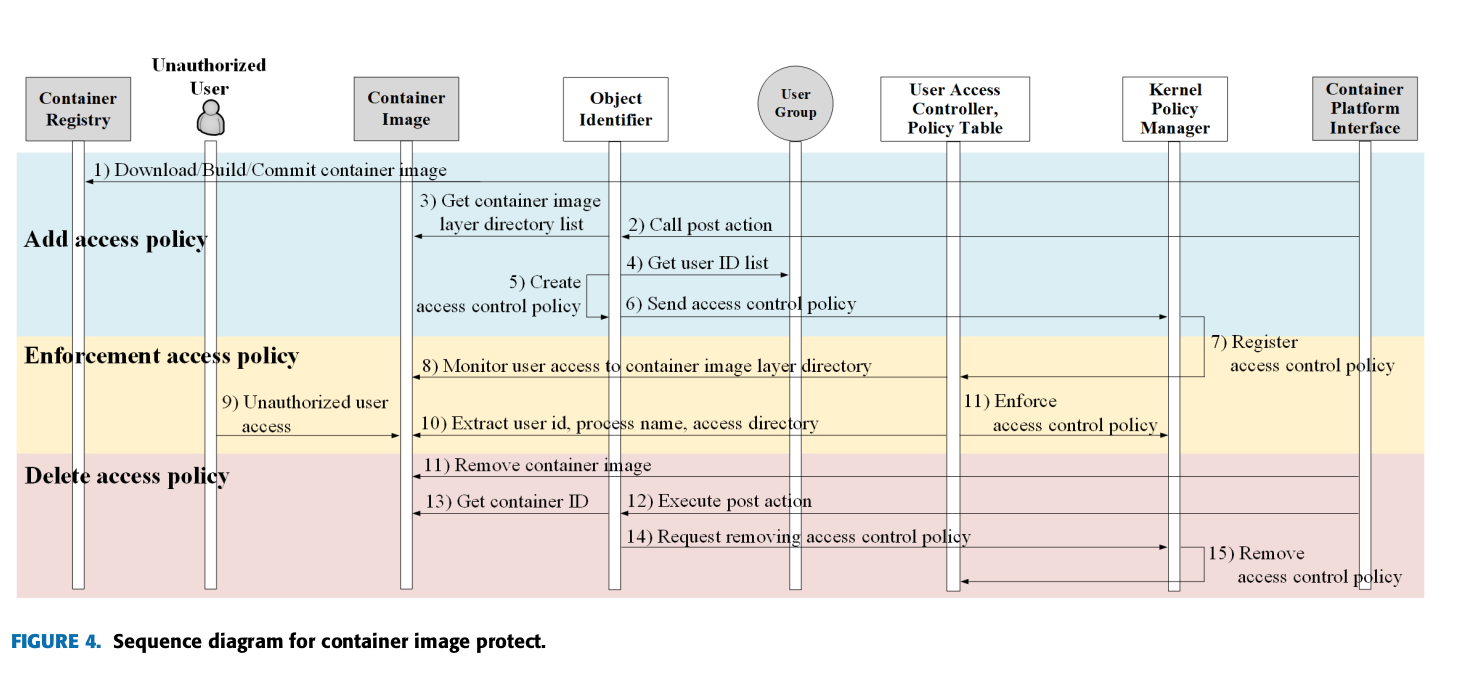
\includegraphics[width=\textwidth]{access_sequence_diagram.png}\cite{Access_Control_Architecture}
\end{frame}

% ======================Current progress============================

\section{Current progress}
\begin{frame}
    \frametitle{Application of MOST}
    \begin{itemize}
        \item \makebox[3cm]{Papers: \hfill} \progressbar[width=5cm,heightr=1,filledcolor=red,
                  emptycolor=blue!30]{0.58333333333} 0.583
        \item \makebox[3cm]{FIXME: \hfill} \progressbar[width=5cm,heightr=1,filledcolor=red,
                  emptycolor=blue!30]{0.308} 0.308
        \item \makebox[3cm]{Pages: \hfill} \progressbar[width=5cm,heightr=1,filledcolor=red,
                  emptycolor=blue!30]{0.38} 0.380
        \item \makebox[3cm]{Expectation: \hfill} \progressbar[width=5cm,heightr=1,filledcolor=red,
                  emptycolor=blue!30]{0} Empty
    \end{itemize}
\end{frame}

\section{Reference}
\begin{frame}[t, allowframebreaks]
    \frametitle{References}
    \printbibliography
\end{frame}

\end{document}